%% LyX 2.3.2 created this file.  For more info, see http://www.lyx.org/.
%% Do not edit unless you really know what you are doing.
\documentclass[12pt,oneside,english]{amsart}
\usepackage[T1]{fontenc}
\usepackage[latin9]{inputenc}
\usepackage{geometry}
\geometry{verbose,tmargin=1.5in,bmargin=1.5in,lmargin=1in,rmargin=1in}
\setlength{\parskip}{\bigskipamount}
\setlength{\parindent}{0pt}
\usepackage{amsthm}
\usepackage{amssymb}

\makeatletter
%%%%%%%%%%%%%%%%%%%%%%%%%%%%%% Textclass specific LaTeX commands.
\numberwithin{equation}{section}
\numberwithin{figure}{section}
\theoremstyle{plain}
\newtheorem{thm}{\protect\theoremname}
\theoremstyle{remark}
\newtheorem{rem}[thm]{\protect\remarkname}

%%%%%%%%%%%%%%%%%%%%%%%%%%%%%% User specified LaTeX commands.
\usepackage{tikz}
\usepackage{xcolor}
\usepackage{babel}
\usepackage{fancyhdr}


\pagestyle{fancy}
\fancyhf{}
\fancyhead[CO]{Dirichlet Landscapes}
\fancyhead[CE]{}
\fancyhead[RO,LE]{\thepage}

\setlength{\headheight}{12pt}

%\captionsetup{tableposition=top,figureposition=bottom,font=small}
\topmargin=-0mm 
\textheight=220mm 
\textwidth=154mm 
\oddsidemargin=5mm

\newcommand{\textoverline}[1]{$\overline{\mbox{#1}}$}

\date{\today}

\author{Jonathan Atwell}
%\address{Stanford GSB}
%\email{jatwell@stanford.edu}
%\thanks{blabla}

\makeatother

\usepackage{babel}
\providecommand{\remarkname}{Remark}
\providecommand{\theoremname}{Theorem}

\begin{document}
\title{Dirichlet Landscapes}
\maketitle

\section{Defining the Dirichlet Dot Product Landscape}

Let the fitness landscape be defined as follows. Let $\lambda\in\Lambda\subseteq\mathbb{R}^{N}$
be a location on the landscape and $X\sim Dir(\alpha)$ be an $N$-dimensional
random vector on the sample space $\Omega$. Consider a state $\omega\in\Omega$,
we denote by $x_{i}=X_{i}(\omega)$ a realization of the $i$-th random
variable in $X$ and, accordingly, $x=\left(x_{1},\dots,x_{N}\right)$
is a realization of $X$. In what follows we restrict our analysis
to the case $\Lambda=\left\{ 0,1\right\} ^{N}$, that is, where the
set of possible locations on the landscape is discrete and corresponds
to the set of the $2^{N}$ edges of an $N$-th dimensional hypercube.

\newcommand{\Depth}{3} 
\newcommand{\Height}{3} 
\newcommand{\Width}{3} 
\begin{figure}[!htb] 
\begin{center}

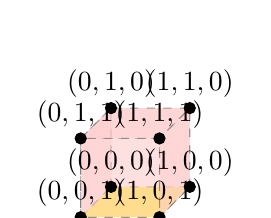
\begin{tikzpicture}

\coordinate (O) at (0,0,0); 
\coordinate (A) at (0,\Width,0); 
\coordinate (B) at (0,\Width,\Height); 
\coordinate (C) at (0,0,\Height); 
\coordinate (D) at (\Depth,0,0); 
\coordinate (E) at (\Depth,\Width,0); 
\coordinate (F) at (\Depth,\Width,\Height); 
\coordinate (G) at (\Depth,0,\Height);




\draw[dashed,gray,fill=yellow!80] (O) -- (C) -- (G) -- (D) -- cycle;% Bottom Face \draw[dashed,gray,fill=blue!30] (O) -- (A) -- (E) -- (D) -- cycle;% Back Face 
\draw[dashed,gray,fill=red!10] (O) -- (A) -- (B) -- (C) -- cycle;% Left Face 
\draw[dashed,gray,fill=red!20,opacity=0.8] (D) -- (E) -- (F) -- (G) -- cycle;% Right Face 
\draw[dashed,gray,fill=red!20,opacity=0.6] (C) -- (B) -- (F) -- (G) -- cycle;% Front Face 
\draw[dashed,gray,fill=red!20,opacity=0.8] (A) -- (B) -- (F) -- (E) -- cycle;% Top Face


\node [thick,above] at (0,0,0) 					{$(0,0,0)$}; 
\node [thick,above] at (0,\Width,0)				{$(0,1,0)$}; 
\node [thick,above] at (0,\Width,\Height)			{$(0,1,1)$}; 
\node [thick,above] at (0,0,\Height)				{$(0,0,1)$}; 
\node [thick,above] at (\Depth,0,0)				{$(1,0,0)$}; 
\node [thick,above] at (\Depth,\Width,0)			{$(1,1,0)$}; 
\node [thick,above] at (\Depth,\Width,\Height)	{$(1,1,1)$}; 
\node [thick,above] at (\Depth,0,\Height)		{$(1,0,1)$};

\filldraw[black] (0,0,0) circle (2pt); 
\filldraw[black] (0,\Width,0) circle (2pt); 
\filldraw[black] (0,\Width,\Height) circle (2pt);
\filldraw[black] (0,0,\Height) circle (2pt);
\filldraw[black] (\Depth,0,0) circle (2pt);
\filldraw[black] (\Depth,\Width,0) circle (2pt);
\filldraw[black] (\Depth,\Width,\Height) circle (2pt);
\filldraw[black] (\Depth,0,\Height) circle (2pt);

\end{tikzpicture}
\caption{The set $\Lambda$ of locations when $N=3$}

\end{center}
\end{figure}

We define the fitness $f$ of a given location as 
\begin{align*}
f: & \Lambda\rightarrow\mathbb{R^{+}}\\
f: & \lambda\mapsto\lambda\cdot x
\end{align*}

This definition of fitness, on the one hand, allows to conceive the
performance of a given configuration as a convex combination of the
values of its dimensions: this conveys the idea that not all dimensions
contribute equally to fitness. On the other hand, an \emph{indirect}\footnote{A direct notion of tradeoff would be embedded by constraining the
total number of resources to be allocated.} idea of tradeoff can also be inferred by this formulation: at any
fixed number of non-zero dimensions, the fact that different dimensions
contribute differently may direct search with the aim of remaining
at least at the same value of fitness.
\begin{rem}
Note that this setup prescribes the use of a unique Dirichlet random
vector to determine the value of the random weights at every location
of the landscape. Another possibility is that of considering a different
random vector be assigned to each different locations. This operationalization
would translate the consideration that importance of the various dimensions
can change as one moves from a location to another one.\footnote{Note that this reasoning can be akin to the idea of inconsistency
of preferences in decision theory.}\emph{@@This setup was used in the original note -- I think it's
an interesting extension but I suggest to first clarify what happens
when weights are ``location-independent''.@@$\hfill\square$}

Marginal contributions (or the \emph{added value}) of each dimension
to fitness can be naturally defined in this setup by considering the
contribution of the focal dimension to total fitness. Formally, let
$f_{i}(\lambda_{i})$ denote the section of the fitness function at
the $i$-th dimension. The contribution of dimension $i$ to fitness
is defined as

\[
\Delta^{i}=f_{i}(1)-f_{i}(0)
\]

which isolates the variation in overall fitness as dimension $i$
varies from $0$ to $1$.\footnote{Note that the definition extends also to the case of multi-valued
coordinates and to the continuous case.}

\textbf{About interdependence and complementarities --} Our definition
of fitness is in accordance with the NK modeling literature in Management
in that it maintains the assumption of fitness be \textbf{increasing
in all of the components} of the $N$-dimensional vector of locations
coordinates. However, this hypothesis makes it hard to explore negative
complementarities without imposing a polynomial functional form for
fitness (Rahmandad, 2019).

In fact, the ``microeconomics-way'' of defining complementarities
(also exploited in Rahmandad, 2019) is through cross-derivatives of
the fitness function (the sign of the cross derivatives dictates the
direction of the complementarity between dimensions). This direction
is not pursuable in this setup due to the definition of the fitness
function (all cross-derivatives are null here).

In this setting, interdependence between dimensions is also indirect,
as opposed to the NK-landscape framework, and derives from the nature
of the Dirichlet weights.

A possible solution is to let not only the weights, but also the locations
coordinates, be random. In particular we can model the coordinates
locations as Bernoulli random variables. Interdependence among them
can then me modeled through the use of a copula. This construction
not only allows to tune interdependence between variables more directly
than in the NK-landscape framework, but also allows to obtain an indirect
study of complementarities between dimensions. In fact, the structure
of correlation between dimensions embeds considerations of mutual
change in the location coordinates. Due to the assumption of monotonicity
of the fitness function, this can be interpreted as two components
being synergetic or antagonistic, in probabilistic terms.
\end{rem}

\end{document}
